\chapter{Reti Neurali}

\section{Introduzione}
\begin{flushleft}
In questo capitolo ci addentreremo nello studio delle reti neurali, iniziando dall'elemento più semplice, il \textbf{percettrone}, e proseguendo verso la costruzione di reti più complesse.
Verranno approfonditi concetti già introdotti nel Capitolo~1, come le funzioni di attivazione, essenziali per introdurre non linearità nei modelli, e i metodi basati sul gradiente per l'ottimizzazione dei parametri, compresa l'inizializzazione dei pesi e altre tecniche fondamentali per garantire un apprendimento efficace. 

Questa trattazione fornirà le basi teoriche necessarie per comprendere pienamente i capitoli successivi, in cui verrà presentata la rete MLP impiegata negli esperimenti di questa tesi. 
\end{flushleft}

\section{Concetti Fondamentali delle Reti Neurali}
\begin{flushleft}
    Le reti neurali artificiali costituiscono una classe di modelli computazionali ispirati al funzionamento dei sistemi nervosi biologici. Sebbene rappresentino una notevole semplificazione rispetto alla complessità delle reti neurali naturali, esse si dimostrano efficaci nella risoluzione di problemi complessi di intelligenza artificiale, dalla classificazione automatica di dati al riconoscimento di pattern sofisticati.

    L'unità computazionale fondamentale è il \textbf{percettrone}, il quale riceve molteplici segnali di input, li elabora attraverso funzioni di attivazione non lineari e genera un output. La comunicazione tra neuroni avviene mediante collegamenti pesati, denominati pesi sinaptici, che memorizzano informazioni apprese e determinano l'intensità dell'influenza che un neurone esercita sui successivi. Questa architettura integra strettamente memoria e capacità di calcolo, consentendo alla rete di apprendere automaticamente dai dati e di adattarsi dinamicamente a nuovi input.
    
    Una caratteristica distintiva delle reti neurali è il parallelismo computazionale: numerosi neuroni elaborano simultaneamente i segnali, creando un sistema distribuito di processori elementari ma coordinati. Questo approccio permette di affrontare problemi di elevata complessità senza la necessità di programmare esplicitamente ogni aspetto della soluzione, sfruttando invece la capacità emergente della rete di identificare pattern e relazioni nei dati.
    
    Storicamente, i primi modelli risalgono a McCulloch e Pitts (1943) con il neurone binario, seguiti dalle prime idee di apprendimento di Hebb (1949). Il perceptrone di Rosenblatt (1958) introdusse pesi variabili, rendendo possibile l'apprendimento, ma la sua limitata capacità portò a un periodo di stagnazione della ricerca fino agli anni '80. La generalizzazione ai problemi non linearmente separabili fu resa possibile dall'algoritmo di retropropagazione (BP) sviluppato da Rumelhart, Hinton e Williams (1986), che utilizza la discesa del gradiente per aggiornare i pesi in funzione dell'errore tra output desiderato e output effettivo.
    Oggi, le reti neurali a più livelli (MLP) addestrate con BP sono largamente impiegate in applicazioni di visione artificiale, elaborazione del linguaggio e sistemi intelligenti, grazie alla loro capacità di generalizzare da esempi e affrontare compiti complessi.
\end{flushleft}

\section{Il percettrone}
\begin{flushleft}
Il percettrone è l'elemento base di processo delle reti neurali artificiali e rappresenta il fondamento teorico su cui si basano i moderni sistemi di machine learning. Proposto per la prima volta da Frank Rosenblatt nel 1957, questo modello matematico è ispirato al funzionamento dei neuroni biologici e costituisce la più semplice forma di neurone artificiale.

\newpage
\subsection{Struttura e Funzionamento}
Il percettrone ha molti input, che possono essere forniti dall'ambiente o essere output di altri percettroni. Associato ad ogni input $x_{j} \in \mathbb{R},j = 1,....,d$, c'è un valore chiamato peso sinaptico $w_{j} \in \mathbb{R}$, e l'output $y$, nel caso più semplice è una somma pesata degli input:
\[
 \hspace{0.5cm} y=\sum_{j=1}^{d} w_j x_j + w_0
\]
Il termine $w_0$ è l'intercetta (o bias) che rende il modello più generale, ed è generalmente modellato come un peso proveniente da un'unità di bias extra,$x_0$, la quale assume sempre il valore $+1$.

\begin{figure}[h!]
\centering
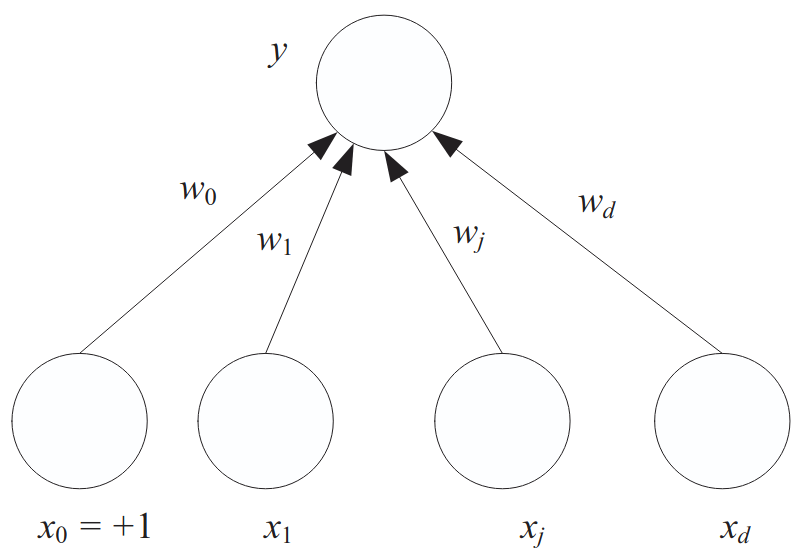
\includegraphics[width=0.4\textwidth]{img/single_perceptron.png}
\caption{Singolo percettrone.  Immagine tratta da \cite{Introduction_to_Machine_Learning_book}}
\label{fig:singolo percettrone}
\end{figure}

\subsection{Funzione di Attivazione}
Nella sua formulazione classica, il percettrone utilizza una funzione di attivazione a soglia (step function) per produrre l'output finale:
\[
\hat{y} = \begin{cases} 
1 & \text{se } y \geq \theta \\
0 & \text{se } y < \theta
\end{cases}
\]
dove $\theta$ è la soglia di attivazione. Questa funzione determina se il neurone si attiva o meno in base al valore della combinazione lineare degli input.

\newpage
\subsection{Interpretazione Geometrica}
Dal punto di vista geometrico, il percettrone definisce un iperpiano nello spazio degli input. L'equazione $\sum_{j=1}^{d} w_j x_j + w_0 = 0$ rappresenta infatti un iperpiano di dimensione $d-1$ in uno spazio $d$-dimensionale. I pesi $w_j$ determinano l'orientamento dell'iperpiano, mentre il bias $w_0$ ne determina la posizione. Il percettrone classifica i punti dello spazio assegnandoli a una delle due classi in base a quale lato dell'iperpiano si trovano.

\subsection{Limitazioni del Percettrone Singolo}
Il percettrone singolo presenta alcune limitazioni fondamentali:
\begin{itemize}
\item \textbf{Linearità}: Può risolvere solo problemi linearmente separabili, ovvero quelli in cui le classi possono essere separate da un iperpiano lineare.
\item \textbf{Funzioni non rappresentabili}: Non può rappresentare funzioni logiche semplici come XOR, che richiedono una separazione non lineare.
\item \textbf{Capacità espressiva limitata}: La sua capacità di apprendimento è limitata a pattern lineari nei dati.
\end{itemize}


\subsection{Algoritmo di Apprendimento}
L'algoritmo di apprendimento del percettrone è un processo iterativo che aggiorna i pesi in base agli errori di classificazione:
\begin{enumerate}
\item Inizializzare i pesi con valori casuali piccoli
\item Per ogni esempio di training $(x^{(i)}, t^{(i)})$:
\begin{itemize}
\item Calcolare l'output $\hat{y}^{(i)}$
\item Se $\hat{y}^{(i)} \neq t^{(i)}$, aggiornare i pesi:
\[w_j := w_j + \eta (t^{(i)} - \hat{y}^{(i)}) x_j^{(i)}\]
dove $\eta$ è il tasso di apprendimento (learning rate)
\end{itemize}
\end{enumerate}

Nonostante le sue limitazioni, il percettrone ha avuto un impatto fondamentale nello sviluppo delle reti neurali artificiali. La comprensione delle sue proprietà e limitazioni ha portato allo sviluppo del percettrone multi-strato (Multi-Layer Perceptron, MLP) e degli algoritmi di backpropagation, che costituiscono la base delle moderne deep neural networks. Il percettrone rimane un modello di riferimento importante per comprendere i principi fondamentali dell'apprendimento automatico e viene ancora utilizzato in applicazioni dove la semplicità e l'interpretabilità sono prioritarie rispetto alla complessità del modello.
\end{flushleft}

\section{Multi-Layer Perceptron}
\begin{flushleft}
Il Multi-Layer Perceptron (MLP) rappresenta l'evoluzione naturale del percettrone singolo per superarne le limitazioni fondamentali. Mentre il percettrone classico può risolvere solo problemi linearmente separabili, l'MLP introduce uno o più livelli nascosti (hidden layers) che conferiscono alla rete la capacità di apprendere relazioni non lineari complesse nei dati.

\subsection{Architettura}
Un MLP è composto da almeno tre tipi di livelli:
\begin{itemize}
\item \textbf{Livello di input}: Riceve i dati dall'ambiente esterno
\item \textbf{Livelli nascosti}: Uno o più livelli intermedi che processano le informazioni
\item \textbf{Livello di output}: Produce la risposta finale della rete
\end{itemize}

Ogni neurone in un livello è completamente connesso a tutti i neuroni del livello successivo, da cui il termine "fully connected" o "dense layer". Per un livello $l$ con $n^{(l)}$ neuroni, l'output del neurone $i$ è dato da:
\[
z_i^{(l)} = \sum_{j=1}^{n^{(l-1)}} w_{ij}^{(l)} a_j^{(l-1)} + b_i^{(l)}
\]
\[
a_i^{(l)} = f(z_i^{(l)})
\]
dove $w_{ij}^{(l)}$ sono i pesi, $b_i^{(l)}$ sono i bias, $a_j^{(l-1)}$ sono le attivazioni del livello precedente e $f(\cdot)$ è la funzione di attivazione.


\begin{figure}[h!]
    \centering
    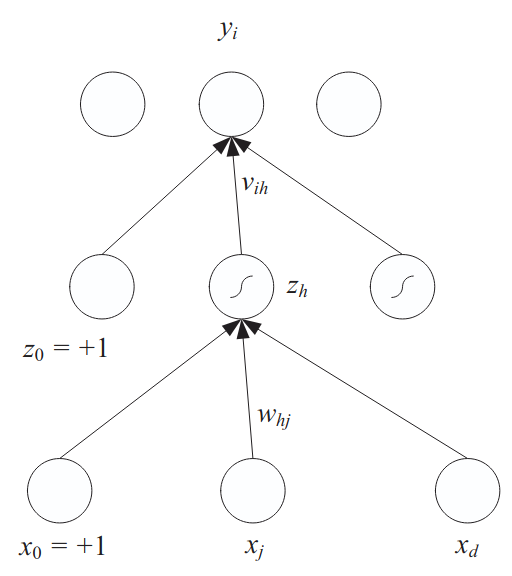
\includegraphics[width=0.4\textwidth]{img/Multi-Layer-Perceptron.png}
    \caption{Architettura Multi Layer Perceptrom. Immagine tratta da \cite{Introduction_to_Machine_Learning_book}}
    \label{fig: Architettura Multi Layer Perceptrom}
\end{figure}
    
\newpage
\subsection{Funzioni di Attivazione Non Lineari}
A differenza del percettrone classico che utilizza una funzione d'attivazione a soglia, l'MLP impiega funzioni di attivazione non lineari e differenziabili, essenziali per l'apprendimento tramite backpropagation. Le più comuni includono:
\begin{itemize}
\item \textbf{Sigmoide}: $f(x) = \frac{1}{1 + e^{-x}}$
\item \textbf{Tanh}: $f(x) = \frac{e^x - e^{-x}}{e^x + e^{-x}}$
\item \textbf{ReLU}: $f(x) = \max(0, x)$
\end{itemize}

\subsection{Funzione Softmax per Classificazione Multi-classe}
Nel livello di output per problemi di classificazione multi-classe, viene spesso utilizzata la funzione softmax, che trasforma un vettore di valori reali in una distribuzione di probabilità:
\[
\text{softmax}(z_i) = \frac{e^{z_i}}{\sum_{j=1}^K e^{z_j}}
\]
dove $z_i$ è l'input del neurone $i$ e $K$ è il numero totale di classi.

Le proprietà fondamentali della softmax sono:
\begin{itemize}
\item \textbf{Normalizzazione}: $\sum_{i=1}^K \text{softmax}(z_i) = 1$
\item \textbf{Monotonicità}: Preserva l'ordinamento relativo degli input
\item \textbf{Differenziabilità}: Essenziale per il calcolo dei gradienti
\end{itemize}

La softmax è particolarmente efficace quando combinata con la cross-entropy loss, formando una coppia matematicamente elegante per l'ottimizzazione. A differenza della funzione sigmoide, che è utilizzata per classificazione binaria, la softmax estende naturalmente il concetto a problemi multi-classe, garantendo che l'output rappresenti una distribuzione di probabilità valida su tutte le possibili classi.


\subsection{Teorema di Approssimazione Universale}
Un risultato teorico fondamentale stabilisce che un MLP con un singolo livello nascosto di dimensione sufficientemente grande può approssimare qualsiasi funzione continua con precisione arbitraria. Questo teorema, dimostrato da Cybenko (1989) e Hornik (1991), fornisce la base teorica per la capacità espressiva delle reti neurali.

\end{flushleft}

\section{Backpropagation}
\begin{flushleft}
L'algoritmo di backpropagation, sviluppato da Rumelhart, Hinton e Williams nel 1986, risolve il problema fondamentale di come addestrare reti neurali multi-strato. L'idea centrale consiste nel calcolare il gradiente della funzione di costo rispetto ai pesi della rete propagando l'errore all'indietro attraverso i livelli.


\subsection{Derivazione Matematica}
Consideriamo una funzione di costo $J(\theta)$ dove $\theta$ rappresenta tutti i parametri della rete. L'obiettivo è minimizzare $J$ aggiornando i pesi secondo la regola:
\[
w_{ij}^{(l)} := w_{ij}^{(l)} - \eta \frac{\partial J}{\partial w_{ij}^{(l)}}
\]

Utilizzando la regola della catena, il gradiente può essere scomposto come:
\[
\frac{\partial J}{\partial w_{ij}^{(l)}} = \frac{\partial J}{\partial z_i^{(l)}} \frac{\partial z_i^{(l)}}{\partial w_{ij}^{(l)}} = \delta_i^{(l)} a_j^{(l-1)}
\]

dove $\delta_i^{(l)} = \frac{\partial J}{\partial z_i^{(l)}}$ è l'errore del neurone $i$ nel livello $l$.

Per il livello di output:
\[
\delta_i^{(L)} = \frac{\partial J}{\partial a_i^{(L)}} f'(z_i^{(L)})
\]

Per i livelli nascosti, l'errore si propaga all'indietro:
\[
\delta_i^{(l)} = \left(\sum_{k=1}^{n^{(l+1)}} w_{ki}^{(l+1)} \delta_k^{(l+1)}\right) f'(z_i^{(l)})
\]

\subsection{Algoritmo di Gradient Descent}
Il gradient descent è l'algoritmo di ottimizzazione fondamentale utilizzato con backpropagation, e ha la seguente struttura:

\begin{enumerate}
\item \textbf{Forward pass}: Calcola le attivazioni per tutti i livelli
\item \textbf{Calcolo del costo}: Valuta la funzione di costo sull'output
\item \textbf{Backward pass}: Calcola i gradienti propagando l'errore all'indietro
\item \textbf{Aggiornamento parametri}: $\theta := \theta - \eta \nabla_\theta J$
\end{enumerate}

Le varianti principali includono:
\begin{itemize}
\item \textbf{Batch Gradient Descent}: Utilizza l'intero dataset per ogni aggiornamento
\item \textbf{Stochastic Gradient Descent (SGD)}: Aggiorna i pesi utilizzando un singolo esempio
\item \textbf{Mini-batch Gradient Descent}: Compromesso che utilizza piccoli batch di dati
\end{itemize}

\subsection{Algoritmo Adam}
Adam (Adaptive Moment Estimation) è un algoritmo di ottimizzazione avanzato che combina i vantaggi di AdaGrad e RMSprop. Mantiene medie mobili esponenziali sia del gradiente che del suo quadrato:

\begin{align}
m_t &= \beta_1 m_{t-1} + (1 - \beta_1) g_t \\
v_t &= \beta_2 v_{t-1} + (1 - \beta_2) g_t^2 \\
\hat{m}_t &= \frac{m_t}{1 - \beta_1^t} \\
\hat{v}_t &= \frac{v_t}{1 - \beta_2^t} \\
\theta_t &= \theta_{t-1} - \frac{\eta}{\sqrt{\hat{v}_t} + \epsilon} \hat{m}_t
\end{align}

dove $g_t$ è il gradiente al tempo $t$, $\beta_1$ e $\beta_2$ sono i fattori di decadimento (tipicamente 0.9 e 0.999), ed $\epsilon$ è una piccola costante per la stabilità numerica.


\subsection{Problema dei Minimi Locali}
I metodi basati sul gradiente presentano diverse sfide teoriche e pratiche:

\begin{itemize}
\item \textbf{Minimi locali}: La funzione di costo può avere molteplici minimi locali dove il gradiente è zero, ma che non rappresentano la soluzione ottimale globale.

\item \textbf{Punti di sella}: In dimensioni elevate, la maggior parte dei punti critici sono punti di sella piuttosto che minimi locali, dove alcune direzioni sono discendenti e altre ascendenti.

\item \textbf{Plateau}: Regioni quasi piatte della superficie di costo dove il gradiente è molto piccolo, causando convergenza lenta.

\item \textbf{Vanishing gradients}: Nei livelli più profondi, i gradienti possono diventare estremamente piccoli, rendendo l'apprendimento inefficace.

\item \textbf{Exploding gradients}: Ib questo caso i gradienti possono crescere esponenzialmente, causando instabilità numerica.
\end{itemize}

Moderne tecniche di regolarizzazione, architetture migliorate e algoritmi di ottimizzazione adattivi aiutano a mitigare questi problemi, rendendo l'addestramento di reti profonde più stabile ed efficace.

\end{flushleft}

\section{Inizializzazione dei Pesi}
\begin{flushleft}
L'inizializzazione dei pesi rappresenta un aspetto critico nell'addestramento delle reti neurali che può determinare il successo o il fallimento del processo di apprendimento. Una cattiva inizializzazione può portare a problemi di vanishing o exploding gradients, convergenza lenta o blocco in minimi locali sfavorevoli.

\subsection{Problematiche dell'Inizializzazione Casuale}
L'inizializzazione naive con valori casuali uniformi o gaussiani può causare diversi problemi:
\begin{itemize}
\item \textbf{Saturazione delle attivazioni}: Valori troppo grandi possono saturare le funzioni di attivazione (es. sigmoide), causando gradienti quasi nulli
\item \textbf{Simmetria}: Inizializzare tutti i pesi con lo stesso valore porta alla perdita della capacità di apprendimento
\item \textbf{Scaling inadeguato}: La varianza delle attivazioni può crescere o diminuire drasticamente attraverso i livelli
\end{itemize}

\subsection{Inizializzazione Xavier/Glorot}
Proposta da Glorot e Bengio (2010), questa tecnica mira a mantenere la varianza delle attivazioni costante attraverso tutti i livelli. Per un livello con $n_{in}$ input e $n_{out}$ output, i pesi sono inizializzati con:

\textbf{Distribuzione uniforme}:
\[
w \sim U\left(-\sqrt{\frac{6}{n_{in} + n_{out}}}, \sqrt{\frac{6}{n_{in} + n_{out}}}\right)
\]

\textbf{Distribuzione normale}:
\[
w \sim \mathcal{N}\left(0, \sqrt{\frac{2}{n_{in} + n_{out}}}\right)
\]

Questa inizializzazione è ottimale per funzioni di attivazione lineari e tanh, mantenendo la varianza delle attivazioni approssimativamente costante durante il forward pass.


\subsection{Inizializzazione He}
Sviluppata da He et al. (2015), questa tecnica è specificamente progettata per funzioni ReLU e loro varianti. Considerando che ReLU azzera metà degli input, la varianza deve essere compensata di conseguenza:

\[
w \sim \mathcal{N}\left(0, \sqrt{\frac{2}{n_{in}}}\right)
\]

Questa inizializzazione tiene conto del fatto che ReLU elimina i valori negativi, mantenendo così una varianza appropriata nel signal propagation.

\subsection{Altre Tecniche di Inizializzazione}
\begin{itemize}
\item \textbf{LeCun initialization}: $w \sim \mathcal{N}(0, \sqrt{1/n_{in}})$, adatta per funzioni SELU
\item \textbf{LSUV (Layer-wise Sequential Unit-Variance)}: Inizializzazione iterativa che normalizza la varianza layer per layer
\end{itemize}

\subsection{Impatto Pratico}
Una corretta inizializzazione può ridurre significativamente il tempo di addestramento e migliorare le prestazioni finali del modello. La scelta del metodo dipende dall'architettura della rete, dalle funzioni di attivazione utilizzate e dalla profondità del modello. Nelle reti moderne, l'inizializzazione He è diventata lo standard per architetture basate su ReLU, mentre Xavier rimane preferita per reti con attivazioni sigmoidi o tanh.

L'importanza dell'inizializzazione è stata ulteriormente evidenziata con lo sviluppo di reti sempre più profonde, dove piccole variazioni nell'inizializzazione possono avere effetti amplificati attraverso molti livelli, influenzando di molto la capacità della rete di apprendere rappresentazioni significative.

\end{flushleft}

\section{Overparametrizzazione delle Reti Neurali}
\begin{flushleft}
L'overparametrizzazione rappresenta uno dei fenomeni più controintuitivi del machine learning moderno, dove le reti neurali sono progettate per avere più parametri di quelli strettamente necessari per rappresentare la funzione target. Questo concetto sfida la saggezza convenzionale del bias-variance trade-off e ha rivoluzionato la comprensione di come le reti neurali apprendono e generalizzano.

\subsection{Il Paradosso della Generalizzazione}
Tradizionalmente, il bias-variance trade-off suggeriva che modelli troppo complessi cadrebbero inevitabilmente in overfitting. Tuttavia, nella pratica moderna, reti neurali con milioni di parametri che interpolano perfettamente i dati di training spesso mostrano eccellenti prestazioni di generalizzazione. Questo fenomeno, noto come \textit{benign overfitting}, indica che nelle reti overparametrizzate il trade-off classico si manifesta in modo diverso: il bias rimane basso mentre la varianza viene controllata attraverso meccanismi di regolarizzazione implicita.

\begin{figure}[h!]
    \centering
    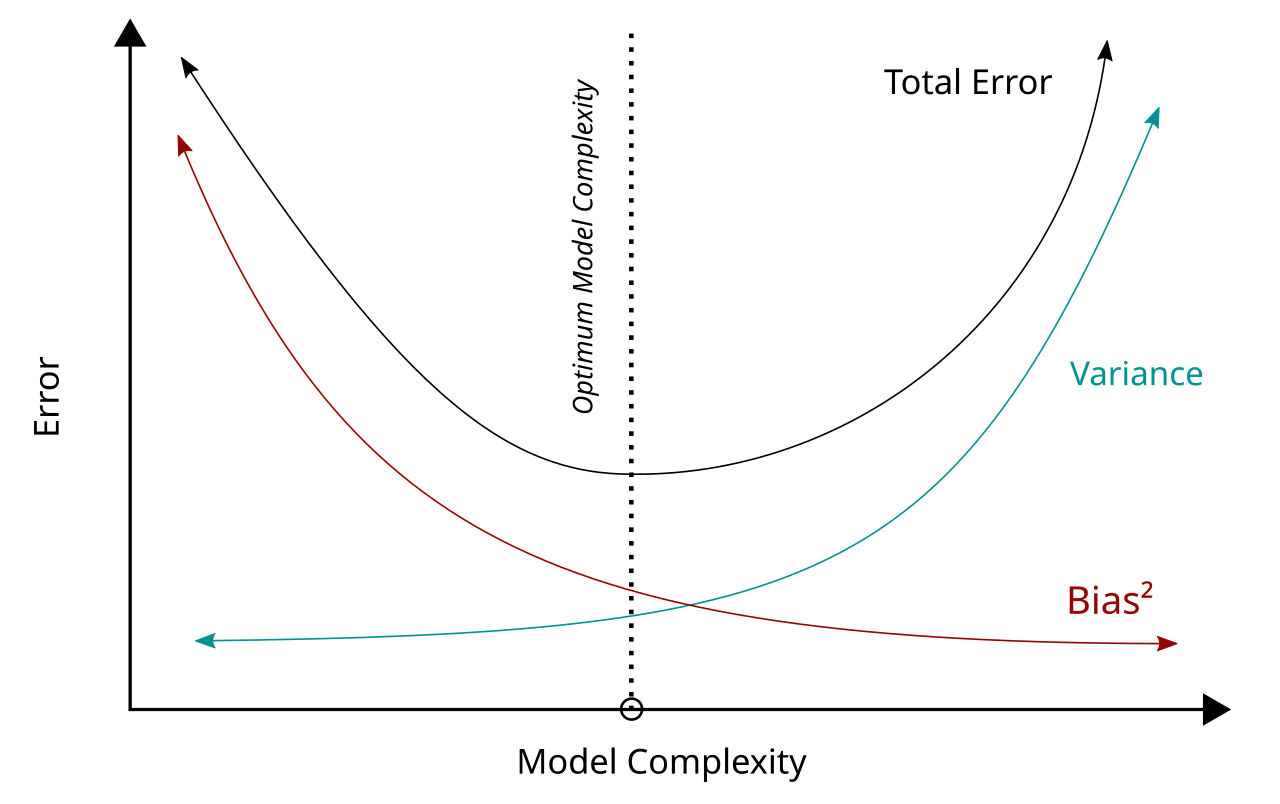
\includegraphics[width=0.6\textwidth]{img/Bias_and_variance_contributing_to_total_error.svg.png}
    \caption{Bias–variance tradeoff. Immagine tratta da \cite{Bias_Variance_Image}}
    \label{fig:Bias–variance tradeoff}
\end{figure}
    
\newpage
\subsection{Il Fenomeno del Double Descent}
Il fenomeno del double descent descrive una curva di rischio che presenta tre regioni distinte:
\begin{enumerate}
\item \textbf{Regime underparameterizzato}: Comportamento classico dove aumentare la complessità migliora le prestazioni fino a un optimum
\item \textbf{Regime critico}: Zona di interpolazione dove il modello fitta perfettamente i dati di training ($\text{Training error} = 0$), spesso con prestazioni di test scadenti
\item \textbf{Regime overparameterizzato}: Oltre la soglia di interpolazione, ulteriori aumenti dei parametri migliorano nuovamente le prestazioni di test
\end{enumerate}

\begin{figure}[h!]
    \centering
    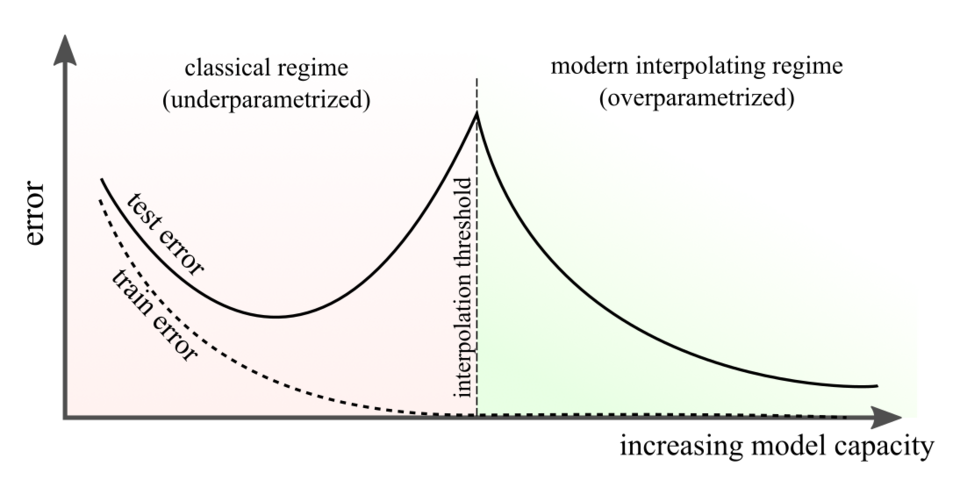
\includegraphics[width=0.7\textwidth]{img/Double_descent.png}
    \caption{Double Descent. Immagine tratta da \cite{Double_Descent_Image}}
    \label{fig:Double Descent}
\end{figure}

\subsection{Differenze tra Reti Piccole e Grandi}
Le dinamiche di apprendimento cambiano drasticamente tra reti di diverse dimensioni:

\subsubsection{Reti Piccole (Underparameterizzate)}
Nelle reti con pochi parametri rispetto alla complessità del problema:
\begin{itemize}
\item \textbf{Sensibilità all'inizializzazione}: La scelta dell'inizializzazione diventa critica poiché lo spazio dei parametri è limitato
\item \textbf{Minimi locali problematici}: Maggior rischio di rimanere bloccati in minimi locali subottimali
\item \textbf{Metodi di ricerca cruciali}: L'algoritmo di ottimizzazione (SGD vs Adam) può fare la differenza tra convergenza e fallimento
\item \textbf{Capacità limitata}: Impossibilità di catturare pattern complessi nei dati
\end{itemize}

\subsubsection{Reti Grandi (Overparameterizzate)}
Nelle reti con molti parametri:
\begin{itemize}
\item \textbf{Robustezza all'inizializzazione}: Meno sensibili alla scelta iniziale dei pesi
\item \textbf{Landscape più favorevole}: Presenza di numerosi minimi locali di qualità simile, spesso connessi attraverso percorsi di bassa perdita
\item \textbf{Regolarizzazione implicita}: Meccanismi intrinseci che prevengono l'overfitting, inclusi il bias induttivo di SGD verso soluzioni con margine ampio e l'effetto regolarizzante del rumore nel gradiente
\item \textbf{Lottery ticket hypothesis}: Esistenza di sotto-reti sparse che mantengono le prestazioni
\end{itemize}

\subsection{Importanza del Metodo di Ricerca}
Nelle reti piccole, il metodo di ottimizzazione assume un ruolo fondamentale: il gradient descent classico può facilmente rimanere intrappolato in minimi locali, mentre algoritmi adattivi come Adam possono aiutare l'esplorazione dello spazio dei parametri. La scelta del learning rate, dello scheduler e della strategia di momentum diventa critica quando i gradi di libertà sono limitati.

Al contrario, nelle reti grandi, diversi algoritmi di ottimizzazione tendono a convergere a soluzioni con prestazioni simili, suggerendo che il landscape di ottimizzazione è intrinsecamente più favorevole. 

L'overparametrizzazione facilita l'ottimizzazione anche per metodi non gradient-based, come gli algoritmi evolutivi, poiché aumenta il numero di configurazioni di parametri che portano a soluzioni accettabili, rendendo lo spazio di ricerca più 'denso' di buone soluzioni.
\end{flushleft}

\section{Conclusioni}
\begin{flushleft}
In questo capitolo sono stati presentati i concetti fondamentali delle reti neurali, che serviranno a comprendere completamente quello che sarà successivamente trattato. Dal percettrone singolo ai Multi-Layer Perceptron, dall'algoritmo di backpropagation alle tecniche di inizializzazione, fino al paradosso dell'overparametrizzazione, questi elementi costituiscono la base teorica e pratica necessaria per affrontare architetture più avanzate e applicazioni specifiche che saranno discusse nei capitoli successivi.
\end{flushleft}